\documentclass[10pt]{ctexart}

%\usepackage{ctex}

\usepackage{geometry}
\geometry{a4paper,scale=0.7}


\usepackage[dvipsnames]{xcolor}
\usepackage{graphicx}
\usepackage{float}
\usepackage{listings}
\usepackage{amsmath}
\usepackage{amssymb}
\usepackage{appendix}

\definecolor{codegreen}{rgb}{0,0.6,0} 
\definecolor{codegray}{rgb}{0.5,0.5,0.5}
\definecolor{codepurple}{rgb}{0.58,0,0.82}
\definecolor{backcolour}{rgb}{0.95,0.95,0.92}

\lstdefinestyle{mystyle}{
    backgroundcolor=\color{backcolour},   
    commentstyle=\color{codegreen},
    keywordstyle=\color{magenta},
    numberstyle=\tiny\color{codegray},
    stringstyle=\color{codepurple},
    basicstyle=\ttfamily\footnotesize,
    breakatwhitespace=false,         
    breaklines=true,                 
    captionpos=b,                    
    keepspaces=true,                 
    numbers=left,                    
    numbersep=5pt,                  
    showspaces=false,                
    showstringspaces=false,
    showtabs=false,                  
    tabsize=2
}

\renewcommand{\lstlistingname}{代码段}
\renewcommand{\lstlistlistingname}{\lstlistingname 索引}
\renewcommand{\listfigurename}{插图索引}


\lstset{style=mystyle}

\setCJKfamilyfont{sy}{Source Han Serif CN}
\newcommand{\name}[1][]{\CJKfamily{sy} 蒋圩淏}

\author{\CJKfamily{sy} 李智聃 \thanks{学号:519021910131,电子邮箱:hyjrgslm-lzd@sjtu.edu.cn}\quad
\CJKfamily{sy} 蒋圩淏 \thanks{学号:519021911045,电子邮箱:weihao.jiang@sjtu.edu.cn} }


\date{}
\title{编译原理实验报告} 

\usepackage{hyperref}
\hypersetup{hidelinks} 

\begin{document}
\maketitle
\tableofcontents 
\section{实验概述}
\subsection*{实验名称}

编译原理大作业实验

\subsection*{实验目的}

\begin{enumerate}
\item 理解算符优先文法,并编写程序,通过类BNF的文法输入得到对应的算符优先分析表。
\item 熟悉TVM框架,并通过TVM框架提供的操作原语,实现在llvm上的卷积计算优化。
\end{enumerate}

\subsection*{分工情况}

{\CJKfamily{sy}实验的完成与每一个人都紧密相关。其中,蒋圩淏主要完成实验的基础部分,李智聃主要完成实验的加分项部分。双方都在对方对应的项目中做出贡献。}

\subsection*{实验结果}

基础部分实现了一个有较高健壮性的算符优先分析表生成器,这个分析表不但能够分析正确的文法,对于错误的文法、不规范的文法和有二义性的文法也有对应的处理与错误提示。

加分项中,使用TVM框架实现了对卷积计算的高性能优化,不论是小规模还是大规模的输入都能够得到较好的优化。

加分项的优化结果表格

\begin{table}[H]
    \centering
    \begin{tabular}{c|c|c|c}
    \hline
    输入大小和输出大小                                                                                          & 优化前的时间           & 优化后的时间          & 提升效率   \\ \hline
    \begin{tabular}[c]{@{}c@{}}n, ic, ih, iw = 1, 3, 32, 32\\ oc, kh, kw = 32, 3, 3\end{tabular}       & 0.104413 ms      & 0.016186 ms     & 91.2\% \\ \hline
    \begin{tabular}[c]{@{}c@{}}n, ic, ih, iw = 100, 512, 32, 32\\ oc, kh, kw = 1024, 3, 3\end{tabular} & 505076.882729 ms & 16044.837527 ms & 96.8\% \\ \hline
    \end{tabular}
\end{table} 
\section{基础部分:算符优先文法分析器}

\subsection{实验环境}

\begin{table}[H]
  \centering
  \begin{tabular}{c|c|c|c|c}
  \hline
  操作系统      & 架构      & 内核版本    & 编程语言   & 解释器版本           \\ \hline
  GNU/Linux & x86\_64 & 5.12.13-2 & Python & 3.9.5 (CPython实现) \\ \hline
  \end{tabular}
\end{table}

因为采用了\texttt{enum.auto}等语言特性,代码至少需要Python 3.6以上版本才能够运行。

\subsection{实验设计}

本实验可以简单分为两个部分:一个是解析类BNF的文法并转化成能够处理的语法形式,一个是对算符优先文法进行判定并生成优先级表。

\subsubsection{类BNF解析}

BNF是推导规则的集合,推导规则写为:

\begin{equation}\nonumber
  <symbol>\quad \rightarrow\quad \_\_expression\_\_
\end{equation}

其中,\texttt{\_\_expression\_\_} 为产生式,由一个或多个符号串组成。符号串间用分隔符$\mid$连接。没有出现在推导规则右侧的符号称为终结符。符号串可以为空,此时我们使用标记$\epsilon$表示。可以用BNF表述一个上下文无关文法。

一个表述的例子为:

\begin{lstlisting}[caption=一个BNF的例子,escapeinside={(*}{*)}]
A -> B C | D
   | E
B -> A | E | F | (* $\epsilon $*)
\end{lstlisting}

\subsubsection*{词法分析}

为了在不改变示例的文法例子的同时又能够接受更广泛的文法,我们补充规定语素间要以空格字符为分隔。例如连在一起的\texttt{BC|}被认为是一个新的符号,而不是\texttt{B}和\texttt{C}的串接与一个分隔符\texttt{|}。我们用简单的字符串操作创建一个词法分析器。

\begin{lstlisting}[caption=词法分析,\texttt{BNFUtils.lex.lex},escapeinside={(*}{*)},language=python]
def lex(string: str) -> list[(IDType, str)]:
    lex_result = []
    induct = "->"
    branch = "|"
    epsilon = "(*$\epsilon$*)"
    token_list = string.split()
    for item in token_list:
        if item == induct:
            lex_result.append((IDType.INDUCT, ""))
            continue
        if item == branch:
            lex_result.append((IDType.BRANCH, ""))
            continue
        if item == epsilon:
            lex_result.append((IDType.EPSILON, ""))
            continue
        lex_result.append((IDType.SYMBOL, item))
    lex_result.append((IDType.DOLLAR, ""))
    return lex_result
\end{lstlisting}

\subsubsection*{语法分析}

我们随即可以用上述的词法单元给出给出描述BNF的BNF范式。

\begin{lstlisting}[caption=BNF的BNF范式,escapeinside={(*}{*)}]
S -> E | E S
E -> SYMBOL INDUCT L
L -> X | L BRANCH X
X -> T | EPSILON
T -> SYMBOL | T SYMBOL
\end{lstlisting}

然而我们注意到,因为符号\texttt{S}的移进前看\texttt{SYMBOL}同时是\texttt{T}的规约前看,会产生移进/规约冲突,至少需要LR(2)的解析器才能够看到\texttt{INDUCT}符号。我们因此在词法分析阶段做预处理,将\texttt{SYMBOL}与\texttt{INDUCT}合并(因为BNF表达上下文无关文法,\texttt{INDUCT}前一定只有一个\texttt{SYMBOL})。这样我们就可以用LALR(1)的方式构建我们的解析器。这一步在\texttt{BNFUtils.lex.prepare}函数中进行操作,一部分错误的输入,会在此处被发现,并输出异常。

\begin{lstlisting}[caption=词法分析阶段异常输入示例,escapeinside={(*}{*)}]
Input: A -> -> B
BNFUtils.common.BNFLexStageGrammarError: Wrong representation: A -> ->
\end{lstlisting}

紧接着就是语法分析器以及语法制导翻译的设计。我们希望将文法解析成树的形式,以方便后续的推导。位于\texttt{BNFUtils.LALR\_parse.parse}的语法分析器是Lookahead(1)的一个通用语法分析器,能够通过\texttt{BNFUtils.BNF\_LALR\_const}定义的动作、跳转、规约表完成相应的动作。LR分析器的一趟过程中我们同时完成S属性的语法制导的翻译。在规约时进行相应的操作。下面的规约数组中的每一个元组中的元素分别指代规约动作的表示,规约需要弹出栈的数目,规约结果的类型,和规约的函数。

\begin{lstlisting}[caption=规约数组,\texttt{BNFUtils.BNF\_LALR\_const},language=python]
Reduce = [
    ("S'-> S", 1, GrammarType.Error, lambda s: None),
    ("E -> INDUCT L", 2, GrammarType.E, lambda induct, induct_list: (induct, induct_list)),
    ("L -> X", 1, GrammarType.L, lambda induction: [induction]),
    ("L -> L BRANCH X", 3, GrammarType.L, lambda induct_list, _, induction: induct_list + [induction]),
    ("S -> E", 1, GrammarType.S, lambda sentence: [sentence]),
    ("S -> S E", 2, GrammarType.S, lambda sentence, sentence_list: sentence + [sentence_list]),
    ("T -> SYMBOL", 1, GrammarType.T, lambda t: [t]),
    ("T -> T SYMBOL", 2, GrammarType.T, lambda t_list, t: t_list + [t]),
    ("X -> T", 1, GrammarType.X, lambda t: t),
    ("X -> EPSILON", 1, GrammarType.X, lambda epsilon: epsilon)
]
\end{lstlisting}

LALR分析的过程中,一些错误的输入会在此处被发现,并输出异常。

\begin{lstlisting}[caption=语法分析阶段异常输入示例]
Input:
A -> | E
E -> ( A )

BNFUtils.common.BNFParseStageGrammarError: Grammar not correct.
Error happened at state 3 when parsing.
State 3 performs: E -> INDUCT • L
Current state sentence:
| E E -> ( A ) $
Current state stack:
status(0) A -> status(3)
\end{lstlisting}

\subsubsection*{语义分析}

紧接着进行语义分析。语义分析包含符号表提取和语句处理。通过集合操作筛选出终结符表和非终结符表、指明初始符号,并用数字代替他们,以简化后续的操作,这个操作定义在\texttt{BNFUtils.static.type\_tagging}中。BNF没有规定初始符号。我们按照约定,使用第一行的文法符号作为初始符号。

我们需要对不规范的语句进行处理。其中包括重复的定义和不规范的转写。这些不规范的语句会影响后续内容,增加额外的操作,因此需要进行处理以缩减优化。

\begin{lstlisting}[caption=不规范的语句示例]
重复定义:
E -> A | B A | B A      => E -> A | B A

不规范的转写:
E -> A
E -> B A                => E -> A | B A
\end{lstlisting}

以以下正确但不规范的BNF文法为例,当分析完成时,输出与结果如下。

\begin{lstlisting}[caption=BNF分析结果]
Input:
A -> B A | C
A -> C
B -> C

Output:
WARNING: identical branches found. Removed.

Result:
Grammar tree:
(
  (
    (INDUCT, 0),
    (
      ( (NON_TERMINAL, 1), (NON_TERMINAL, 0) ),
      ( (TERMINAL, 0) )
    )
  ),
  (
    (INDUCT, 1),
    (
      ( (TERMINAL, 0) )
    )
  )
)

terminal:    ['C']
symbol:      ['A', 'B']
init_symbol: A
\end{lstlisting}

\subsubsection{算符优先表生成}

\subsubsection*{算符优先文法文法简介}

算符优先文法的特点是文法的产生式中不含两个相邻的非终结符。其定义如下:

假定G是不含$\epsilon$-产生式的算符文法。对于任何一对终结符$a$, $b$,有:

\begin{itemize}
  \item $a \doteq b$, 如果 $ P \rightarrow^* \alpha a b \beta \in G \lor P \rightarrow^* \alpha a Q b \beta \in G $
  \item $a \lessdot b$, 如果 $ P \rightarrow^* \alpha a R \beta \in G, R  \rightarrow^* b\beta \lor R \rightarrow^* Qb\beta $
  \item $a \gtrdot b$, 如果 $ P \rightarrow^* \alpha R b \beta \in G, R  \rightarrow^* \alpha a \lor R \rightarrow^* \alpha aQ $
\end{itemize}

如果对于任何一对终结符$a$, $b$, 最多满足$a \doteq b, a \lessdot b, a \gtrdot b$三个条件之一,则称为算符优先文法,否则则具有二义性。

\subsubsection*{预处理}

我们先判断这个文法是否是一个算符优先文法。在预处理这一步,我们能够进行的判断是是否存在$\epsilon$-产生式和两个相邻的非终结符。这一步在\texttt{OPGUtils.static.OPG\_check}中展现。

接下来,根据文法的定义,我们需要加入一个推导式 $S' \rightarrow \$ S\$ $,其中S是初始符号,$\$$是标记语句端点的终结符。

\subsubsection*{FIRSTVT,LASTVT表}

在前面对算符之间优先级关系的定义中,我们需要寻找非终结符的首终结符和尾终结符。我们定义以下两个概念:

首终结符集 $FIRSTVT(B) = \{b | B\rightarrow^* b\beta \lor B \rightarrow^* Qb\beta \}$

尾终结符集 $LASTVT(B) = \{b | B\rightarrow^* \beta b \lor B \rightarrow^* \beta bQ \}$

此时可以定义新的终结符关系:

\begin{itemize}
  \item $a \doteq b$, 如果 $ P \rightarrow \alpha a b \beta \in G \lor P \rightarrow \alpha a Q b \beta \in G $
  \item $ P \rightarrow \alpha a R \beta \in G, \forall b \in FIRSTVT(R), a \lessdot b$
  \item $ P \rightarrow \alpha R b \beta \in G,\forall a \in LASTVT(R), a \gtrdot b$
\end{itemize}

而首尾终结符集的构造可以按照定义进行。首先将直接的继承关系引入。

我们通过栈的方式传播更新,来构建首尾终结符集。

\begin{lstlisting}[caption=构建首终结符集,\texttt{OPGUtils.construct}, language=python]
def first_vt(grammar):
    first_vt_table = [set() for _ in range(len(grammar))]
    stack = []

    for induction in grammar:
        for sentence in induction[1]:
            # B -> aβ, a in FIRSTVT(B)
            if sentence[0][0] == IDType.TERMINAL:
                first_vt_table[induction[0][1]].add(sentence[0][1])
                stack.append(induction[0][1])
            # B -> Daβ, a in FIRSTVT(B)
            if len(sentence) > 1 and sentence[0][0] == IDType.NON_TERMINAL and sentence[1][0] == IDType.TERMINAL:
                first_vt_table[induction[0][1]].add(sentence[1][1])
                stack.append(induction[0][1])

    while len(stack):
        non_terminal = stack.pop()
        for induction in grammar:
            for sentence in induction[1]:
                # B -> Dβ, FIRSTVT(D) in FIRSTVT(B)
                if sentence[0][0] == IDType.NON_TERMINAL and sentence[0][1] == non_terminal:
                    if len(first_vt_table[sentence[0][1]].difference(first_vt_table[induction[0][1]])):
                        first_vt_table[induction[0][1]] = first_vt_table[induction[0][1]] | first_vt_table[
                            sentence[0][1]]
                        stack.append(induction[0][1])
                    pass
    return first_vt_table
\end{lstlisting}

首先我们将直接项加入集合中,对于首终结符集即为$B\rightarrow b\beta, B \rightarrow Qb\beta$,并加入传播更新栈。接下来我们更新间接操作。对于栈顶$Q$,如果生成式中有 $B\rightarrow Q\beta $,说明$FIRSTVT(Q) \subset FIRSTVT(B)$。我们通过集合操作,如果更新了$B$则将$B$加入传播更新栈。如此不断更新,当栈清空时,此时便完成了首终结符集。尾终结符集的构造手段类似。

\subsubsection*{构造算符优先级表}

我们可以按照上面的定义,构造我们的算符优先级表。这一步由函数\texttt{OPGUtils.\allowbreak{}filltable.\allowbreak{}fill\_table}实现。在进行的同时我们检查是否存在二义性。如果对于任何一对终结符$a$, $b$, 最多满足$a \doteq b, a \lessdot b, a \gtrdot b$三个条件之一。当此条件冲突时即可判定具有二义性。

\begin{lstlisting}[caption=构造算符优先级表,\texttt{OPGUtils.filltable}, language=python]
def fill_table(table, firstvt, lastvt, grammar):
    def mark(state, a, b):
        if table[a][b] != Priority.undefined and table[a][b] != state:
            raise OPGAmbiguousError("This OPG is ambiguous!")
        table[a][b] = state

    for induction in grammar:
        for sentence in induction[1]:
            for i in range(len(sentence) - 1):
                if sentence[i][0] == IDType.TERMINAL and sentence[i + 1][0] == IDType.TERMINAL:
                    mark(Priority.equal, sentence[i][1], sentence[i + 1][1])
                if sentence[i][0] == IDType.TERMINAL and sentence[i + 1][0] == IDType.NON_TERMINAL:
                    for term in firstvt[sentence[i + 1][1]]:
                        mark(Priority.less, sentence[i][1], term)
                if sentence[i][0] == IDType.NON_TERMINAL and sentence[i + 1][0] == IDType.TERMINAL:
                    for term in lastvt[sentence[i][1]]:
                        mark(Priority.more, term, sentence[i + 1][1])
                if i != len(sentence) - 2 and sentence[i][0] == IDType.TERMINAL and \
                        sentence[i + 2][0] == IDType.TERMINAL and sentence[i + 1][0] == IDType.NON_TERMINAL:
                    mark(Priority.equal, sentence[i][1], sentence[i + 2][1])
    return
\end{lstlisting}

我们使用测试文法进行测试:

\begin{lstlisting}[caption=测试文法1]
E -> E + T | T
T -> T * F | F
F -> ( E ) | id

    *   id  )   (   +   $
*   >   <   >   <   >   >
id  >       >       >   >
)   >       >       >   >
(   <   <   =   <   <
+   <   <   >   <   >   >
$   <   <       <   <   =

进程已结束,退出代码为 0
\end{lstlisting}

\begin{lstlisting}[caption=测试文法2]
E -> E + E | E * E | ( E ) | id 

OPGUtils.common.OPGAmbiguousError: This OPG is ambiguous!

进程已结束,退出代码为 1
\end{lstlisting}

\subsubsection{输入输出}

我们的程序使用命令行界面控制输入输出。命令行参数如下。

\begin{lstlisting}[caption=命令行参数]
usage: OPGAnalysis.py [-h] [-i INPUT_FILE] [-o OUTPUT_FILE] [--need-traceback]

Generate the OPG Table.

optional arguments:
  -h, --help            show this help message and exit
  -i INPUT_FILE, --input-file INPUT_FILE
                        Specify input file.
  -o OUTPUT_FILE, --output-file OUTPUT_FILE
                        Specify output file.
  --need-traceback      Show the traceback when error occurs.
\end{lstlisting}

给出调用示例文法的文法例子:

\begin{lstlisting}[caption=命令行示例]
python ./OPGAnalysis.py -i example/input1.txt -o example/output1.txt
python ./OPGAnalysis.py -i example/input2.txt -o example/output2.txt
\end{lstlisting}

在执行中,不会写入\texttt{example/output2.txt},因为文法是二义性的。

\section{加分部分:TVM框架卷积计算优化}

\subsection{实验环境}

\begin{table}[H]
  \centering
  \begin{tabular}{c|c|c|c|c}
  \hline
  操作系统      & 架构   &  内存  & CPU & 内核版本       \\ \hline
  GNU/Linux & x86\_64 &   8GB  & 2CPU,12核心,24线程  & 5.8.0-53  \\ \hline
  \end{tabular}
\end{table}

\begin{table}[H]
    \centering
    \begin{tabular}{c|c|c|c}
    \hline
    编程语言   & 解释器版本    & TVM框架版本      & LLVM版本   \\ \hline
    Python & 3.8.0 (CPython实现) & 0.8.dev0  & 12.0 \\ \hline
    \end{tabular}
  \end{table}

\subsection{实验设计}

为了执行更加准确的测试,并匹配当前使用的0.8.dev0版TVM,我们修改了原有的脚本,以获取更直观的输出。

\begin{lstlisting}[caption=测试组件示例,language=python]
def main():
    test_suite([1, 3, 32, 32, 32, 3, 3], 1)
    test_suite([100, 512, 32, 32, 1024, 3, 3], 2)
\end{lstlisting}


\subsubsection{小输入部分优化~原始计算内容分析}

调用tvm默认的schedule函数,我们能够得到以下运算的循环表达式。

\begin{lstlisting}[caption=原始循环表达式,在test1.old.ir文件中]
primfn(A_1: handle, B_1: handle, compute_1: handle) -> ()
  attr = {"global_symbol": "main", "tir.noalias": True}
  buffers = {compute: Buffer(compute_2: Pointer(float32), float32, [1, 32, 32, 32], []),
             B: Buffer(B_2: Pointer(float32), float32, [32, 3, 3, 3], []),
             A: Buffer(A_2: Pointer(float32), float32, [1, 3, 32, 32], [])}
  buffer_map = {A_1: A, B_1: B, compute_1: compute} {
  attr [pad_temp: Pointer(float32)] "storage_scope" = "global";
  allocate(pad_temp, float32, [3468]) {
    for (i1: int32, 0, 3) {
      for (i2: int32, 0, 34) {
        for (i3: int32, 0, 34) {
          pad_temp[(((i1*1156) + (i2*34)) + i3)] = @tir.if_then_else(((((1 <= i2) && (i2 < 33)) && (1 <= i3)) && (i3 < 33)), (float32*)A_2[((((i1*1024) + (i2*32)) + i3) - 33)], 0f32, dtype=float32)
        }
      }
    }
    for (ff: int32, 0, 32) {
      for (yy: int32, 0, 32) {
        for (xx: int32, 0, 32) {
          compute_2[(((ff*1024) + (yy*32)) + xx)] = 0f32
          for (rc: int32, 0, 3) {
            for (ry: int32, 0, 3) {
              for (rx: int32, 0, 3) {
                compute_2[(((ff*1024) + (yy*32)) + xx)] = ((float32*)compute_2[(((ff*1024) + (yy*32)) + xx)] + ((float32*)pad_temp[(((((rc*1156) + (yy*34)) + (ry*34)) + xx) + rx)]*(float32*)B_2[((((ff*27) + (rc*9)) + (ry*3)) + rx)]))
              }
            }
          }
        }
      }
    }
  }
}
\end{lstlisting}

运行的时间是0.104413 ms。运行结果参见附录中的图片\textcolor{MidnightBlue}{\ref{1-1}}。可以看到还有很大优化空间。

其中,前一部分pad\_temp是卷积过程中的Padding。通常为了更好地节省内存和缓存占用,我们会将这一部分内联到后续运算中。但TVM提供的卷积包装器并不方便指向内部的阶段,我们此处不采用这种优化手段。有文章指出,对于深度学习中常用的卷积结构,通过likely标记判断过程,这样的优化可以提升约10\%的性能。

对于主要的运算过程compute\_2,不难发现,不经优化的原始运算内容是一次卷积,编译后会在每个要计算的图片上,逐位移动覆盖的卷积核并计算卷积值。编译后的计算表现为一次三重循环(初始化)与一次六重循环(赋值),每次计算一组赋值。在本次优化中,我们仅考虑对六重循环这一主要耗时部分进行优化。

\subsubsection{卷积核循环展开}

我们通过以下的schedule函数来展开卷积核:

\begin{lstlisting}[caption=卷积核循环展开,language=python]
def schedule(output):
    s = tvm.te.create_schedule(output.op)
    s[output].unroll(output.op.reduce_axis[2])
    s[output].unroll(output.op.reduce_axis[1])
    return s
\end{lstlisting}

可以得到新的循环表达式:

\begin{lstlisting}[caption=卷积核展开后的循环表达式]
for (ff: int32, 0, 32) {
  for (yy: int32, 0, 32) {
    for (xx: int32, 0, 32) {
      compute_2[(((ff*1024) + (yy*32)) + xx)] = 0f32
      for (rc: int32, 0, 3) {
        compute_2[(((ff*1024) + (yy*32)) + xx)] = ((float32*)compute_2[(((ff*1024) + (yy*32)) + xx)] + ((float32*)pad_temp[(((rc*1156) + (yy*34)) + xx)]*(float32*)B_2[((ff*27) + (rc*9))]))
        compute_2[(((ff*1024) + (yy*32)) + xx)] = ((float32*)compute_2[(((ff*1024) + (yy*32)) + xx)] + ((float32*)pad_temp[((((rc*1156) + (yy*34)) + xx) + 1)]*(float32*)B_2[(((ff*27) + (rc*9)) + 1)]))
        compute_2[(((ff*1024) + (yy*32)) + xx)] = ((float32*)compute_2[(((ff*1024) + (yy*32)) + xx)] + ((float32*)pad_temp[((((rc*1156) + (yy*34)) + xx) + 2)]*(float32*)B_2[(((ff*27) + (rc*9)) + 2)]))
        compute_2[(((ff*1024) + (yy*32)) + xx)] = ((float32*)compute_2[(((ff*1024) + (yy*32)) + xx)] + ((float32*)pad_temp[((((rc*1156) + (yy*34)) + xx) + 34)]*(float32*)B_2[(((ff*27) + (rc*9)) + 3)]))
        compute_2[(((ff*1024) + (yy*32)) + xx)] = ((float32*)compute_2[(((ff*1024) + (yy*32)) + xx)] + ((float32*)pad_temp[((((rc*1156) + (yy*34)) + xx) + 35)]*(float32*)B_2[(((ff*27) + (rc*9)) + 4)]))
        compute_2[(((ff*1024) + (yy*32)) + xx)] = ((float32*)compute_2[(((ff*1024) + (yy*32)) + xx)] + ((float32*)pad_temp[((((rc*1156) + (yy*34)) + xx) + 36)]*(float32*)B_2[(((ff*27) + (rc*9)) + 5)]))
        compute_2[(((ff*1024) + (yy*32)) + xx)] = ((float32*)compute_2[(((ff*1024) + (yy*32)) + xx)] + ((float32*)pad_temp[((((rc*1156) + (yy*34)) + xx) + 68)]*(float32*)B_2[(((ff*27) + (rc*9)) + 6)]))
        compute_2[(((ff*1024) + (yy*32)) + xx)] = ((float32*)compute_2[(((ff*1024) + (yy*32)) + xx)] + ((float32*)pad_temp[((((rc*1156) + (yy*34)) + xx) + 69)]*(float32*)B_2[(((ff*27) + (rc*9)) + 7)]))
        compute_2[(((ff*1024) + (yy*32)) + xx)] = ((float32*)compute_2[(((ff*1024) + (yy*32)) + xx)] + ((float32*)pad_temp[((((rc*1156) + (yy*34)) + xx) + 70)]*(float32*)B_2[(((ff*27) + (rc*9)) + 8)]))
      }
    }
  }
}
\end{lstlisting}

此部分的运行结果参见附录中的图片\textcolor{MidnightBlue}{\ref{1-2}}。

可以发现,现在每次最内循环都是多次赋值。这样,我们可以减少循环次数,并为接下来的优化打下基础。

\subsubsection{vectorize原语进行向量化计算}

在经过unroll处理后,我们发现每次内层循环的举动都是一系列float32的赋值过程。这一过程中指令相同数据不同,非常适合利用CPU提供的SIMD指令集。因此我们对内层运算添加指令s[output].vectorize(output.op.axis[3]),让内层的赋值运算变为向量形式。运行结果如下:

\begin{lstlisting}[caption=向量化计算后的循环表达式]
for (ff: int32, 0, 32) {
    for (yy: int32, 0, 32) {
      compute_2[ramp(((ff*1024) + (yy*32)), 1, 32)] = broadcast(0f32, 32)
      for (rc: int32, 0, 3) {
            compute_2[ramp(((ff*1024) + (yy*32)), 1, 32)] = ((float32x32*)compute_2[ramp(((ff*1024) + (yy*32)), 1, 32)] + ((float32x32*)pad_temp[ramp(((rc*1156) + (yy*34)), 1, 32)]*broadcast((float32*)B_2[((ff*27) + (rc*9))], 32)))
            compute_2[ramp(((ff*1024) + (yy*32)), 1, 32)] = ((float32x32*)compute_2[ramp(((ff*1024) + (yy*32)), 1, 32)] + ((float32x32*)pad_temp[ramp((((rc*1156) + (yy*34)) + 1), 1, 32)]*broadcast((float32*)B_2[(((ff*27) + (rc*9)) + 1)], 32)))
            compute_2[ramp(((ff*1024) + (yy*32)), 1, 32)] = ((float32x32*)compute_2[ramp(((ff*1024) + (yy*32)), 1, 32)] + ((float32x32*)pad_temp[ramp((((rc*1156) + (yy*34)) + 2), 1, 32)]*broadcast((float32*)B_2[(((ff*27) + (rc*9)) + 2)], 32)))
            compute_2[ramp(((ff*1024) + (yy*32)), 1, 32)] = ((float32x32*)compute_2[ramp(((ff*1024) + (yy*32)), 1, 32)] + ((float32x32*)pad_temp[ramp((((rc*1156) + (yy*34)) + 34), 1, 32)]*broadcast((float32*)B_2[(((ff*27) + (rc*9)) + 3)], 32)))
            compute_2[ramp(((ff*1024) + (yy*32)), 1, 32)] = ((float32x32*)compute_2[ramp(((ff*1024) + (yy*32)), 1, 32)] + ((float32x32*)pad_temp[ramp((((rc*1156) + (yy*34)) + 35), 1, 32)]*broadcast((float32*)B_2[(((ff*27) + (rc*9)) + 4)], 32)))
            compute_2[ramp(((ff*1024) + (yy*32)), 1, 32)] = ((float32x32*)compute_2[ramp(((ff*1024) + (yy*32)), 1, 32)] + ((float32x32*)pad_temp[ramp((((rc*1156) + (yy*34)) + 36), 1, 32)]*broadcast((float32*)B_2[(((ff*27) + (rc*9)) + 5)], 32)))
            compute_2[ramp(((ff*1024) + (yy*32)), 1, 32)] = ((float32x32*)compute_2[ramp(((ff*1024) + (yy*32)), 1, 32)] + ((float32x32*)pad_temp[ramp((((rc*1156) + (yy*34)) + 68), 1, 32)]*broadcast((float32*)B_2[(((ff*27) + (rc*9)) + 6)], 32)))
            compute_2[ramp(((ff*1024) + (yy*32)), 1, 32)] = ((float32x32*)compute_2[ramp(((ff*1024) + (yy*32)), 1, 32)] + ((float32x32*)pad_temp[ramp((((rc*1156) + (yy*34)) + 69), 1, 32)]*broadcast((float32*)B_2[(((ff*27) + (rc*9)) + 7)], 32)))
            compute_2[ramp(((ff*1024) + (yy*32)), 1, 32)] = ((float32x32*)compute_2[ramp(((ff*1024) + (yy*32)), 1, 32)] + ((float32x32*)pad_temp[ramp((((rc*1156) + (yy*34)) + 70), 1, 32)]*broadcast((float32*)B_2[(((ff*27) + (rc*9)) + 8)], 32)))
      }
    }
}
\end{lstlisting}

运行时间是0.056781 ms,运算速度有了较大提升。运行结果参见附录中的图片\textcolor{MidnightBlue}{\ref{1-3}}。

\subsubsection{parallel原语并行执行内部循环}

经过向量化指令,运行速度已经有了较大的提高。但是因为当前运算规模相对较小,我们再对for循环结构进行优化收益已经不大,因此我们考虑增加系统同时运行的计算数量。幸运的是,卷积运行模型中,各个外层运算式中没有数据相关性,因此我们可以放心地添加并行指令。对函数添加指令`s[output].parallel(output.op.axis[1])`,让最外层的for循环变为并行执行。

到此,我们的schedule函数变为

\begin{lstlisting}[caption=小输入部分优化函数,language=python]
def schedule(output):
    s = tvm.te.create_schedule(output.op)
    s[output].parallel(output.op.axis[1])
    s[output].vectorize(output.op.axis[3])
    s[output].unroll(output.op.reduce_axis[2])
    s[output].unroll(output.op.reduce_axis[1])
    return s
\end{lstlisting}

运行结果如下:

\begin{lstlisting}[caption=并行执行后的循环表达式]
for (ff: int32, 0, 32) "parallel" {
  for (yy: int32, 0, 32) {
    compute_2[ramp(((ff*1024) + (yy*32)), 1, 32)] = broadcast(0f32, 32)
    for (rc: int32, 0, 3) {
      compute_2[ramp(((ff*1024) + (yy*32)), 1, 32)] = ((float32x32*)compute_2[ramp(((ff*1024) + (yy*32)), 1, 32)] + ((float32x32*)pad_temp[ramp(((rc*1156) + (yy*34)), 1, 32)]*broadcast((float32*)B_2[((ff*27) + (rc*9))], 32)))
      compute_2[ramp(((ff*1024) + (yy*32)), 1, 32)] = ((float32x32*)compute_2[ramp(((ff*1024) + (yy*32)), 1, 32)] + ((float32x32*)pad_temp[ramp((((rc*1156) + (yy*34)) + 1), 1, 32)]*broadcast((float32*)B_2[(((ff*27) + (rc*9)) + 1)], 32)))
      compute_2[ramp(((ff*1024) + (yy*32)), 1, 32)] = ((float32x32*)compute_2[ramp(((ff*1024) + (yy*32)), 1, 32)] + ((float32x32*)pad_temp[ramp((((rc*1156) + (yy*34)) + 2), 1, 32)]*broadcast((float32*)B_2[(((ff*27) + (rc*9)) + 2)], 32)))
      compute_2[ramp(((ff*1024) + (yy*32)), 1, 32)] = ((float32x32*)compute_2[ramp(((ff*1024) + (yy*32)), 1, 32)] + ((float32x32*)pad_temp[ramp((((rc*1156) + (yy*34)) + 34), 1, 32)]*broadcast((float32*)B_2[(((ff*27) + (rc*9)) + 3)], 32)))
      compute_2[ramp(((ff*1024) + (yy*32)), 1, 32)] = ((float32x32*)compute_2[ramp(((ff*1024) + (yy*32)), 1, 32)] + ((float32x32*)pad_temp[ramp((((rc*1156) + (yy*34)) + 35), 1, 32)]*broadcast((float32*)B_2[(((ff*27) + (rc*9)) + 4)], 32)))
      compute_2[ramp(((ff*1024) + (yy*32)), 1, 32)] = ((float32x32*)compute_2[ramp(((ff*1024) + (yy*32)), 1, 32)] + ((float32x32*)pad_temp[ramp((((rc*1156) + (yy*34)) + 36), 1, 32)]*broadcast((float32*)B_2[(((ff*27) + (rc*9)) + 5)], 32)))
      compute_2[ramp(((ff*1024) + (yy*32)), 1, 32)] = ((float32x32*)compute_2[ramp(((ff*1024) + (yy*32)), 1, 32)] + ((float32x32*)pad_temp[ramp((((rc*1156) + (yy*34)) + 68), 1, 32)]*broadcast((float32*)B_2[(((ff*27) + (rc*9)) + 6)], 32)))
      compute_2[ramp(((ff*1024) + (yy*32)), 1, 32)] = ((float32x32*)compute_2[ramp(((ff*1024) + (yy*32)), 1, 32)] + ((float32x32*)pad_temp[ramp((((rc*1156) + (yy*34)) + 69), 1, 32)]*broadcast((float32*)B_2[(((ff*27) + (rc*9)) + 7)], 32)))
      compute_2[ramp(((ff*1024) + (yy*32)), 1, 32)] = ((float32x32*)compute_2[ramp(((ff*1024) + (yy*32)), 1, 32)] + ((float32x32*)pad_temp[ramp((((rc*1156) + (yy*34)) + 70), 1, 32)]*broadcast((float32*)B_2[(((ff*27) + (rc*9)) + 8)], 32)))
    }
  }
}
\end{lstlisting}

运行时间是0.016186 ms。运行结果参见附录中的图片\textcolor{MidnightBlue}{\ref{1-4}}。可以发现,由于实验系统允许以较多的线程并行执行,并行的增益效果非常显著。

至此,我们完成了对小规模数组的优化工作,优化性能达到了91.2\%。

\subsubsection{大输入部分优化}

调用tvm默认的schedule函数,我们能够得到以下运算的循环表达式。

\begin{lstlisting}[caption=大输入原始循环表达式,在test2.old.ir文件中]
primfn(A_1: handle, B_1: handle, compute_1: handle) -> ()
  attr = {"global_symbol": "main", "tir.noalias": True}
  buffers = {compute: Buffer(compute_2: Pointer(float32), float32, [1, 1024, 32, 32], []),
             B: Buffer(B_2: Pointer(float32), float32, [1024, 512, 3, 3], []),
             A: Buffer(A_2: Pointer(float32), float32, [1, 512, 32, 32], [])}
  buffer_map = {A_1: A, B_1: B, compute_1: compute} {
  attr [pad_temp: Pointer(float32)] "storage_scope" = "global";
  allocate(pad_temp, float32, [591872]) {
    for (i1: int32, 0, 512) {
      for (i2: int32, 0, 34) {
        for (i3: int32, 0, 34) {
          pad_temp[(((i1*1156) + (i2*34)) + i3)] = @tir.if_then_else(((((1 <= i2) && (i2 < 33)) && (1 <= i3)) && (i3 < 33)), (float32*)A_2[((((i1*1024) + (i2*32)) + i3) - 33)], 0f32, dtype=float32)
        }
      }
    }
    for (ff: int32, 0, 1024) {
      for (yy: int32, 0, 32) {
        for (xx: int32, 0, 32) {
          compute_2[(((ff*1024) + (yy*32)) + xx)] = 0f32
          for (rc: int32, 0, 512) {
            for (ry: int32, 0, 3) {
              for (rx: int32, 0, 3) {
                compute_2[(((ff*1024) + (yy*32)) + xx)] = ((float32*)compute_2[(((ff*1024) + (yy*32)) + xx)] + ((float32*)pad_temp[(((((rc*1156) + (yy*34)) + (ry*34)) + xx) + rx)]*(float32*)B_2[((((ff*4608) + (rc*9)) + (ry*3)) + rx)]))
              }
            }
          }
        }
      }
    }
  }
}
\end{lstlisting}

运行时间是505076.882729 ms。运行结果参见附录中的图片\textcolor{MidnightBlue}{\ref{2-1}}。可以看到还有很大优化空间。

我们沿用小输入优化的schedule函数(图\textcolor{MidnightBlue}{\ref{2-2}}),能够得到一个较好的结果,这已经达到了优化的要求。

但是我们发现,卷积核的filter较大。因为filter是一个线性的组成,如果我们能够将filter调换顺序,把大的filter调换到外部,可以增加程序的局部性。

\begin{lstlisting}[caption=最终优化函数,language=python]
def schedule(output):
    s = tvm.te.create_schedule(output.op)
    if output.op.reduce_axis[0].dom.extent > output.op.axis[3].dom.extent:
        s[output].reorder(output.op.axis[0], output.op.axis[1], output.op.reduce_axis[0], output.op.axis[2],
                          output.op.axis[3])
    s[output].parallel(output.op.axis[1])
    s[output].vectorize(output.op.axis[3])
    s[output].unroll(output.op.reduce_axis[2])
    s[output].unroll(output.op.reduce_axis[1])
    return s
\end{lstlisting}

运行结果如下:

\begin{lstlisting}[caption=大输入优化循环表达式,在test2.opt.ir文件中]
for (ff: int32, 0, 1024) "parallel" {
    for (yy.init: int32, 0, 32) {
    compute_2[ramp(((ff*1024) + (yy.init*32)), 1, 32)] = broadcast(0f32, 32)
    }
    for (rc: int32, 0, 512) {
    for (yy: int32, 0, 32) {
        compute_2[ramp(((ff*1024) + (yy*32)), 1, 32)] = ((float32x32*)compute_2[ramp(((ff*1024) + (yy*32)), 1, 32)] + ((float32x32*)pad_temp[ramp(((rc*1156) + (yy*34)), 1, 32)]*broadcast((float32*)B_2[((ff*4608) + (rc*9))], 32)))
        compute_2[ramp(((ff*1024) + (yy*32)), 1, 32)] = ((float32x32*)compute_2[ramp(((ff*1024) + (yy*32)), 1, 32)] + ((float32x32*)pad_temp[ramp((((rc*1156) + (yy*34)) + 1), 1, 32)]*broadcast((float32*)B_2[(((ff*4608) + (rc*9)) + 1)], 32)))
        compute_2[ramp(((ff*1024) + (yy*32)), 1, 32)] = ((float32x32*)compute_2[ramp(((ff*1024) + (yy*32)), 1, 32)] + ((float32x32*)pad_temp[ramp((((rc*1156) + (yy*34)) + 2), 1, 32)]*broadcast((float32*)B_2[(((ff*4608) + (rc*9)) + 2)], 32)))
        compute_2[ramp(((ff*1024) + (yy*32)), 1, 32)] = ((float32x32*)compute_2[ramp(((ff*1024) + (yy*32)), 1, 32)] + ((float32x32*)pad_temp[ramp((((rc*1156) + (yy*34)) + 34), 1, 32)]*broadcast((float32*)B_2[(((ff*4608) + (rc*9)) + 3)], 32)))
        compute_2[ramp(((ff*1024) + (yy*32)), 1, 32)] = ((float32x32*)compute_2[ramp(((ff*1024) + (yy*32)), 1, 32)] + ((float32x32*)pad_temp[ramp((((rc*1156) + (yy*34)) + 35), 1, 32)]*broadcast((float32*)B_2[(((ff*4608) + (rc*9)) + 4)], 32)))
        compute_2[ramp(((ff*1024) + (yy*32)), 1, 32)] = ((float32x32*)compute_2[ramp(((ff*1024) + (yy*32)), 1, 32)] + ((float32x32*)pad_temp[ramp((((rc*1156) + (yy*34)) + 36), 1, 32)]*broadcast((float32*)B_2[(((ff*4608) + (rc*9)) + 5)], 32)))
        compute_2[ramp(((ff*1024) + (yy*32)), 1, 32)] = ((float32x32*)compute_2[ramp(((ff*1024) + (yy*32)), 1, 32)] + ((float32x32*)pad_temp[ramp((((rc*1156) + (yy*34)) + 68), 1, 32)]*broadcast((float32*)B_2[(((ff*4608) + (rc*9)) + 6)], 32)))
        compute_2[ramp(((ff*1024) + (yy*32)), 1, 32)] = ((float32x32*)compute_2[ramp(((ff*1024) + (yy*32)), 1, 32)] + ((float32x32*)pad_temp[ramp((((rc*1156) + (yy*34)) + 69), 1, 32)]*broadcast((float32*)B_2[(((ff*4608) + (rc*9)) + 7)], 32)))
        compute_2[ramp(((ff*1024) + (yy*32)), 1, 32)] = ((float32x32*)compute_2[ramp(((ff*1024) + (yy*32)), 1, 32)] + ((float32x32*)pad_temp[ramp((((rc*1156) + (yy*34)) + 70), 1, 32)]*broadcast((float32*)B_2[(((ff*4608) + (rc*9)) + 8)], 32)))
    }
    }
}
\end{lstlisting}

运行结果参见附录中的图片\textcolor{MidnightBlue}{\ref{2-3}}。

此时我们的运行时间是16044.837527 ms,优化性能达到了96.8\%。

%\include{tests.tex}

\section{总结与感想}

本次实验的基础部分,我们实现了一个有较高健壮性的算符优先分析表生成器,这个分析表不但能够分析正确的文法,对于错误的文法、不规范的文法和有二义性的文法也有对应的处理与错误提示。

本次实验的加分项中,我们使用TVM框架实现了对卷积计算的高性能优化,不论是小规模还是大规模的输入都能够得到较好的优化。

\begin{itemize}
    \item 对于知识点的准确掌握。课程和教程中的知识点都比较空泛,有一个较为抽象的理解,但是对于具体的操作,仍然要实践出真知。通过本次实验,我们对于算符优先文法和TVM的各种优化原语都有了较深刻的理解。
    \item 环境的配置。TVM框架仍然处于孵化阶段,版本之间的API差异比较大,而且版本之间对于LLVM的依赖不同,与其他成熟的框架相比,文档、示例、编译都比较欠缺,除了与GitHub同步的0.8.dev0版本,其他代码都无法正确变异。通过认真翻阅API文档,我们完成了环境配置,并在此基础上完成了实验。
    \item 团队的协作。因为本项目并非是能够拆分的传统项目,对于团队的协作提出了较大的挑战性。我们使用git进行版本的迭代和团队的协作,并通过GitLab提供的Worker功能进行持续集成,对程序的正确性进行实时判断,尤其是第二个项目,耗时较长,使用CI/CD和自动化测试后,程序的开发效率得到了很好的提升。
\end{itemize}

通过本次编译原理大作业的学习,我们对于算符优先文法、TVM框架,和深度学习中的矩阵计算优化手段都有了更好的理解。编译器以其牵一发而动全身的地位,算法的设计尤为重要。此次通过重温实现经典算法、探索深度学习编译器的优化前沿,对于我们普通程序的编写和优化也是大有裨益的。

编译原理的课时很短,因为课程进度的设计原因,在课堂教学中,对于编译器的近代进展只是蜻蜓点水。感谢蒋力老师与助教们的精心设计与辛勤付出,为我们提供了这样一个难得的机会。最后要感谢上海交通大学,为我们提供了这样一门精彩纷呈的课程。
\appendix
\section*{附录}
\section{图片}
\pagenumbering{roman}

\begin{figure}[H]
    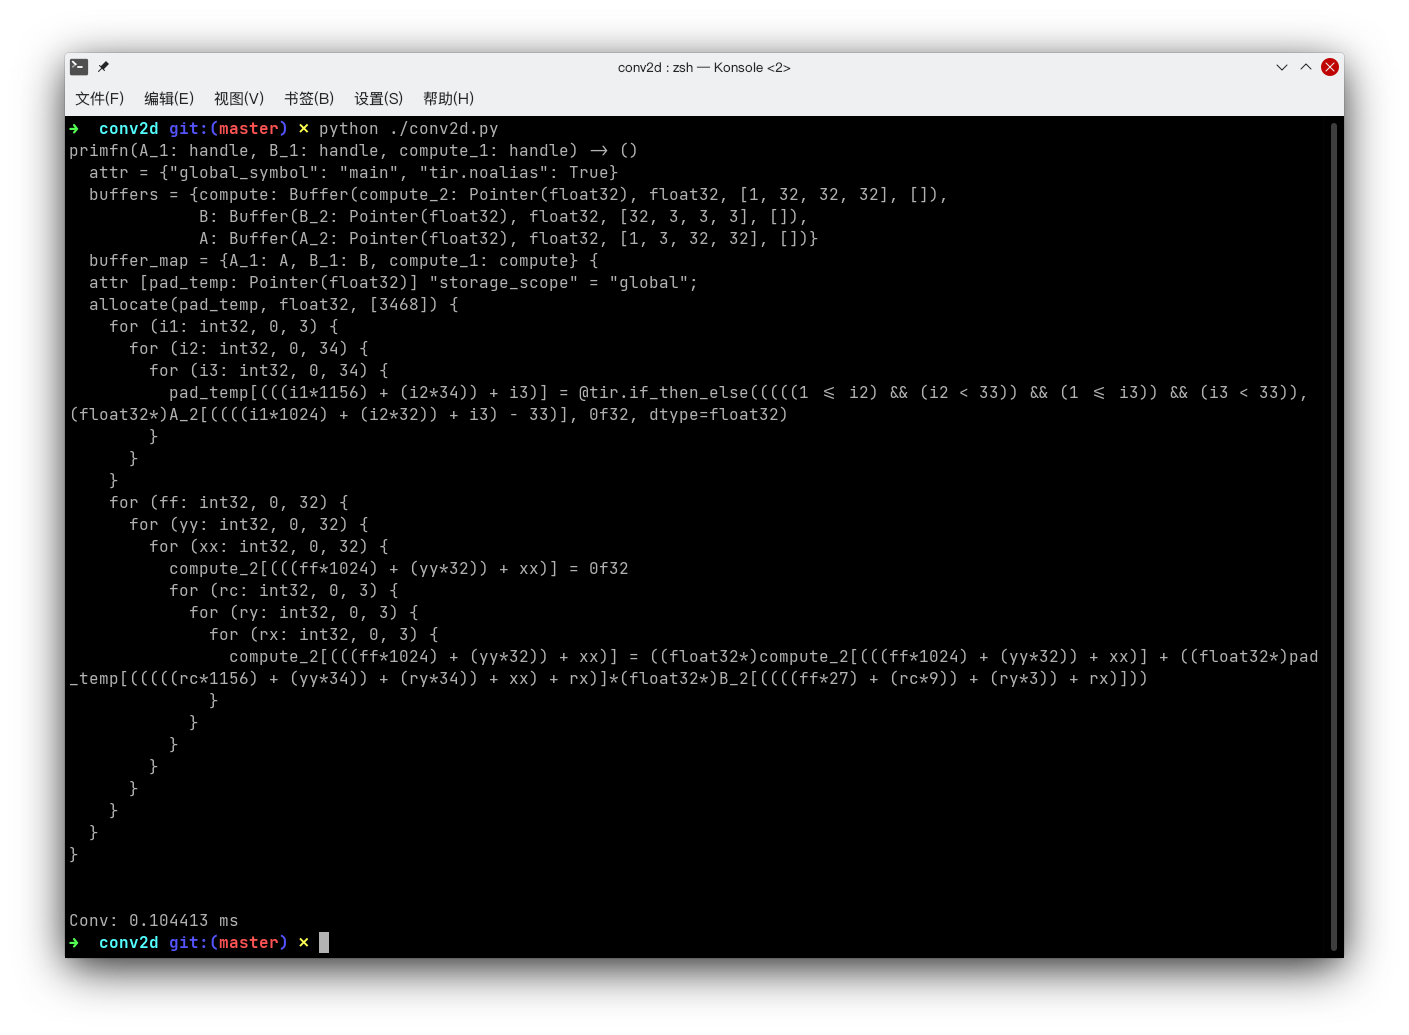
\includegraphics[width=\textwidth]{images/orig-1.png}
    \caption{小输入部分~原始计算内容}\label{1-1}
\end{figure}

\begin{figure}[H]
    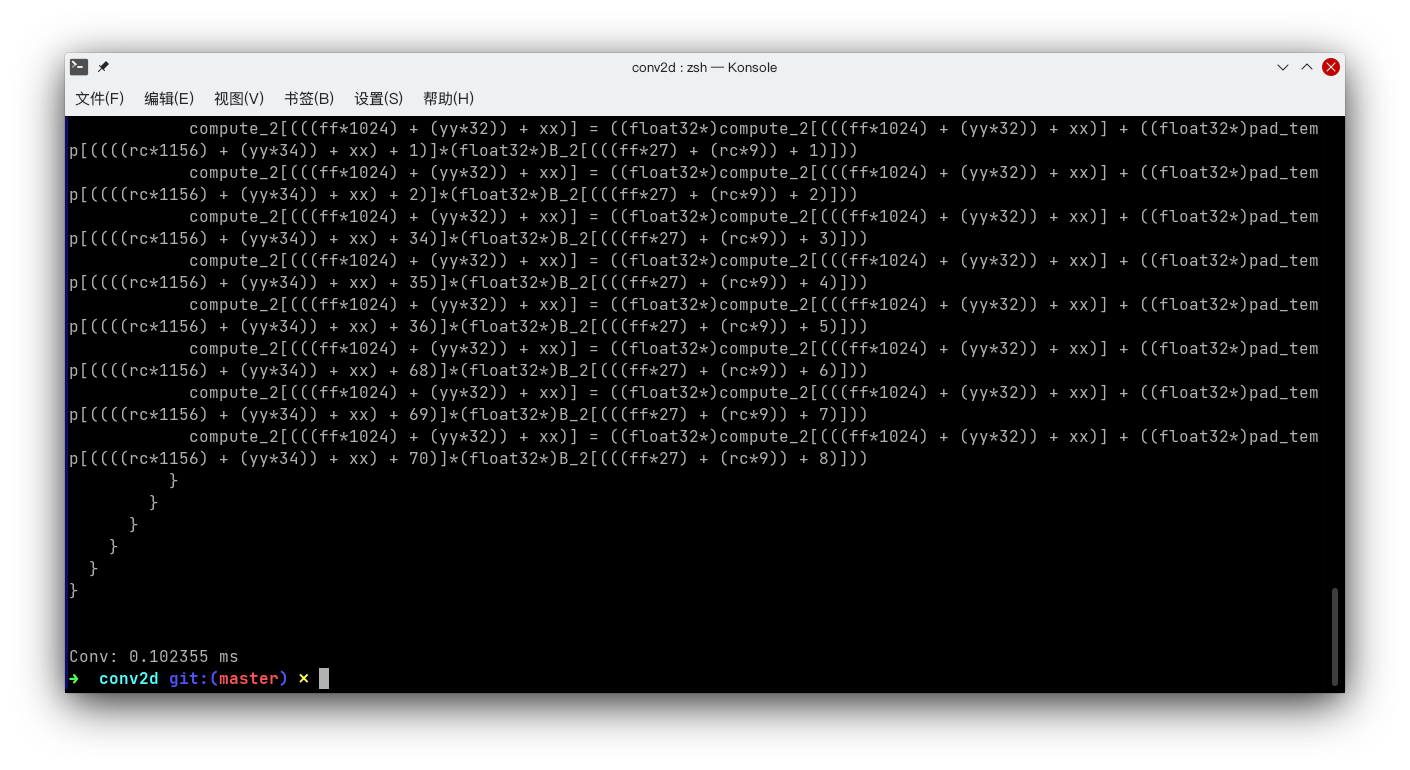
\includegraphics[width=\textwidth]{images/orig-2.png}
    \caption{小输入部分~卷积核循环展开}\label{1-2}
\end{figure}

\begin{figure}[H]
    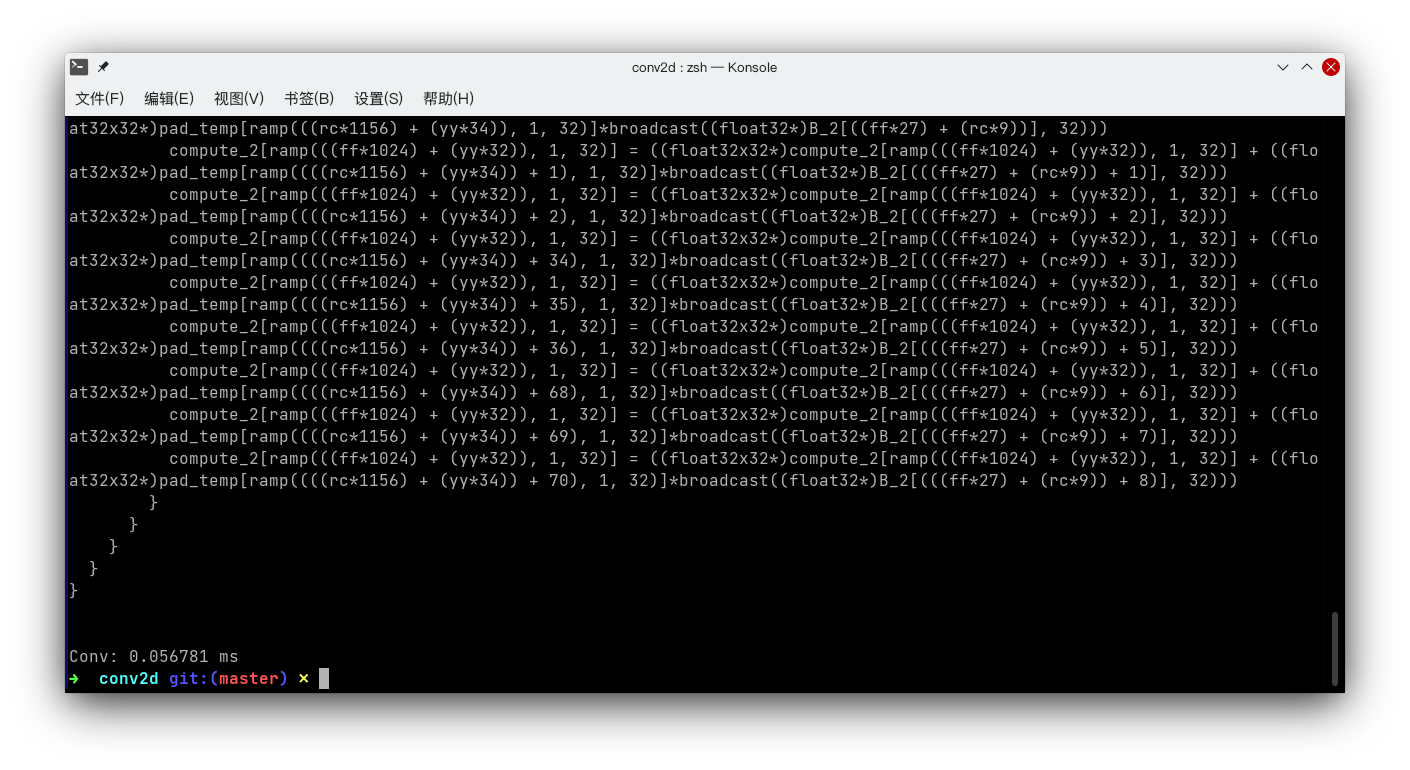
\includegraphics[width=\textwidth]{images/orig-3.png}
    \caption{小输入部分~向量化计算}\label{1-3}
\end{figure}

\begin{figure}[H]
    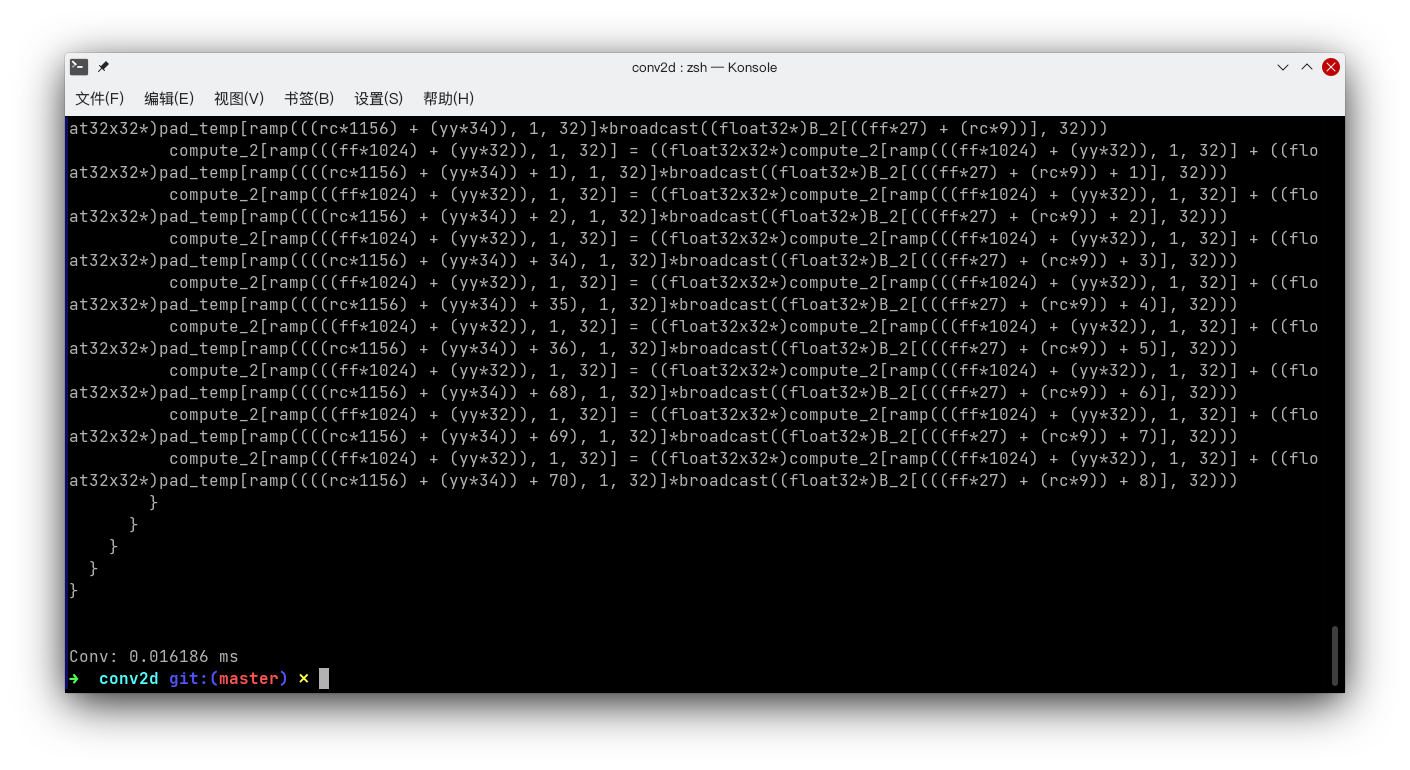
\includegraphics[width=\textwidth]{images/orig-4.png}
    \caption{小输入部分~并行执行}\label{1-4}
\end{figure}

\begin{figure}[H]
    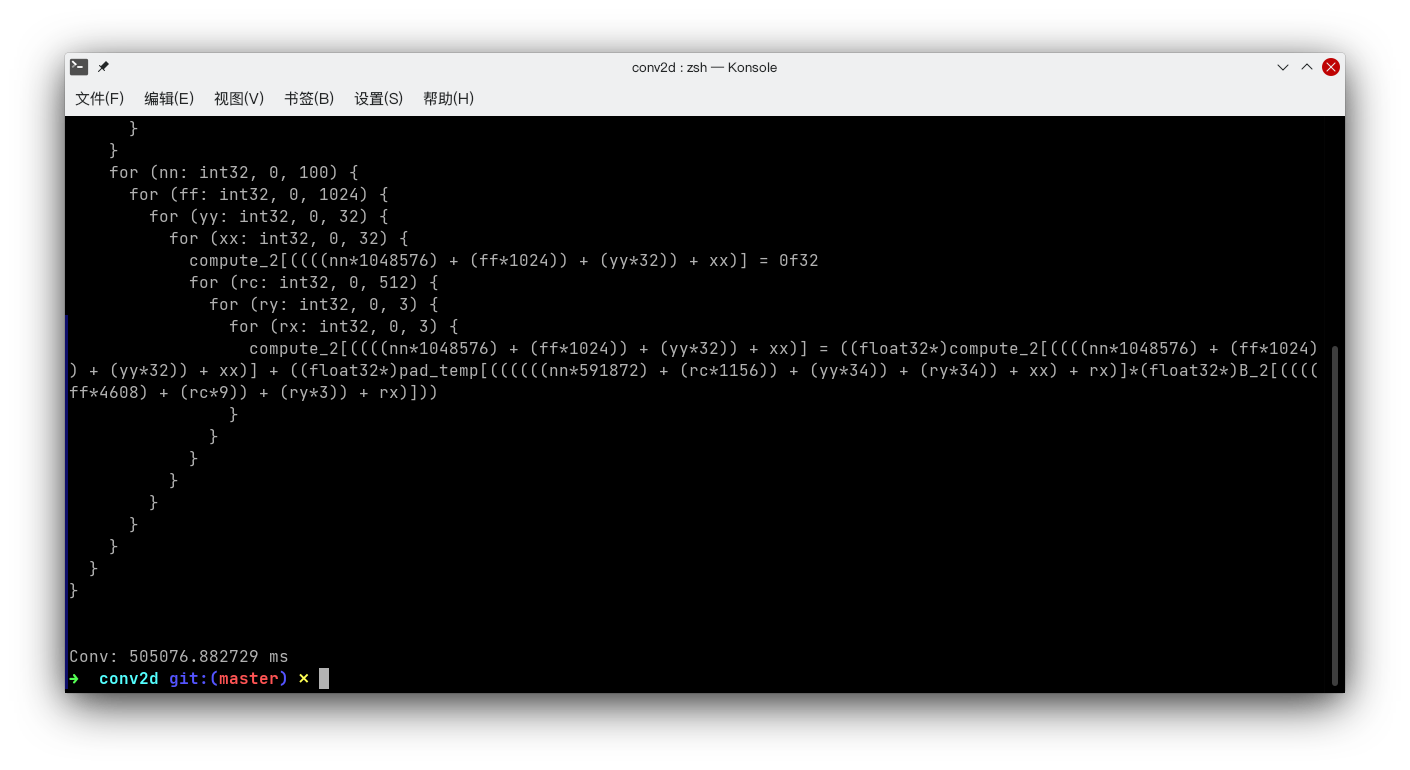
\includegraphics[width=\textwidth]{images/orig2-1.png}
    \caption{大输入部分~原始计算内容}\label{2-1}
\end{figure}
\begin{figure}[H]
    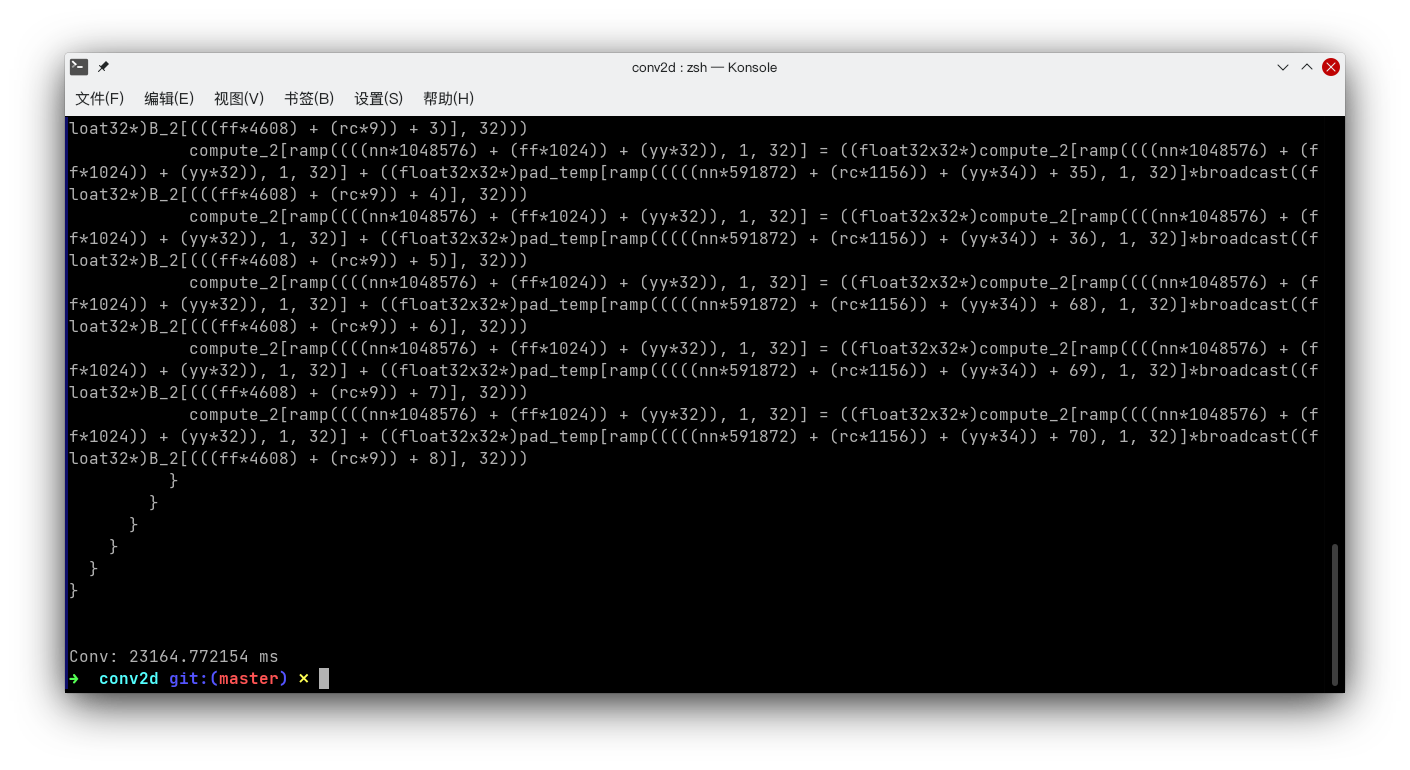
\includegraphics[width=\textwidth]{images/orig2-2.png}
    \caption{大输入部分~使用小输入优化}\label{2-2}
\end{figure}
\begin{figure}[H]
    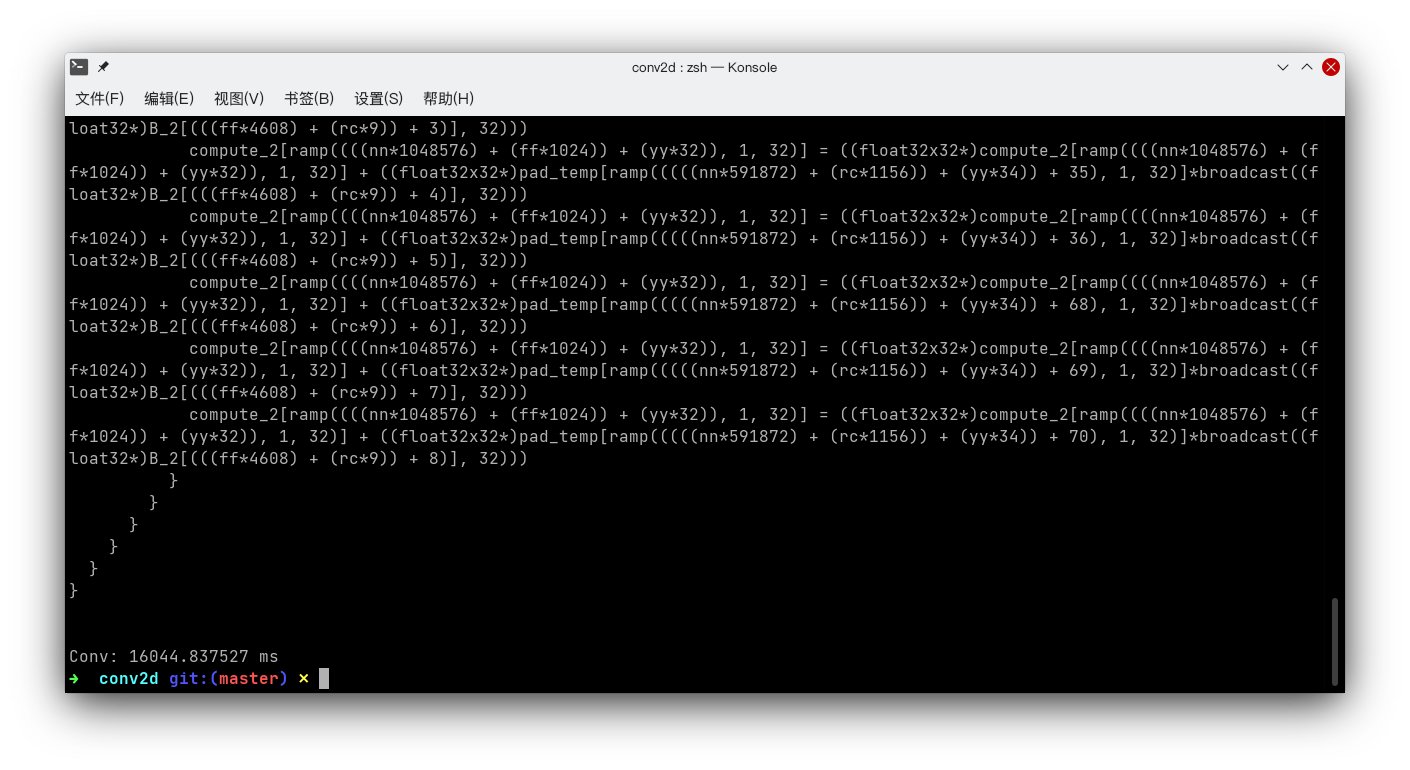
\includegraphics[width=\textwidth]{images/orig2-3.png}
    \caption{大输入部分~交换次序}\label{2-3}
\end{figure}

\addcontentsline{toc}{section}{代码段索引}
\lstlistoflistings
\addcontentsline{toc}{section}{插图索引}
\listoffigures
\end{document}
